\chapter{Introduction}
Measuring environmental parameters in and around the water in Greenland (or any coastal nation) is a time consuming task. Today measurements are carried out by manually navigating large vessels up and down along the coastline and into the fjords. 

An example where this could be highly efficient would be at the Fukushima accident 2011. As seen on figure \ref{img:fukushimaradiation} there exists no measurements of the radiation in the water, due to the danger and resource demand of sending a manned expedition. Only estimates of the radiation level in the water exist, and therefore it is impossible to say what effects the radiation have had on the surrounding maritime life, as well as what proximity margin should exist. A fleet of small autonomous vessels would be able to quickly give an overview of the damage caused, as well as the spread and strength of the radiation.
\mimg{0.3\textwidth}{img/fukushima.pdf}{At the site of the 2011 Fukushima accident only landside radiation measurements exist}{img:fukushimaradiation}
Another purpose of these measurements, which will be the primary focus for this project, could be to measure the water depth for bathymetric surveys \cite{StweartOceanography}. This would allow for safer voyages in and around the coastlines, and for general environmental studies. 

These measurements are today carried out by one large vessel, which could be exchanged for several smaller ones to reduce the surveying time and labor cost. This would make for a faster measurement of the coastline as well as giving an opportunity to measure previously un-surveyed waters due to costs. 

Reducing the size of a vessel, poses some other challenges in regards to the weather conditions and other environmental parameters, that has a much larger influence on small scale vessels, than on larger ones.
Limitations are also imposed from the availability of power for the boats,  the noise of measurements as well as limitations on the availability of computing power and communication links. This paper will deal with how such a surveying vessel can be developed, and still measure the water depth whilst under the influence of the above.

A challenge using a single beam transducer to measure water depth is the roll/pitch of the craft. Figure \vref{fig:beamer} illustrates this problem, where an induced pitch of the ship (eg. a wave) makes it impossible for the vessel to make a precise measurement.

\begin{figure}[h]
\centering
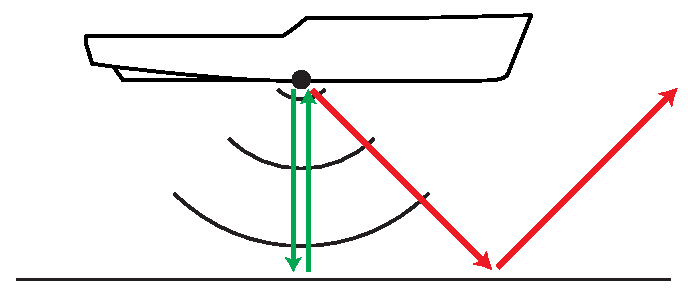
\includegraphics[width=0.5\textwidth]{img/beamer}
\caption{Overview of a depth mapping system. The green represents a measurement shot directly down and the red represents a measurement with induced pitch on the ship}
\label{fig:beamer}
\end{figure}

Another challenge, using a fleet of measurement boats, would be how to enable them all to coordinate and effectivize their effort. This could be done by having a mothership which would be in charge of coordinating and controlling the smaller ships. This larger ship would be able to store larger amount of energy, and be able to charge the smaller ships as needed. Due to this easy access to power it would be able to turn up signal strength and computing power as needed. This way it would be possible to reduce the requirements for the hardware aboard the ships, while still having sufficient hardware to compute complex algorithms necessary for control. Having this process centralized, however, offers some additional challenges. Packetloss and limited communicationspeed demand a robust system where these conditions are addressed. In this project the effect of packetloss and limited available data is analyzed and a solution based on an implementation of a kalman filter is suggested.
